\documentclass[10pt,a4paper]{amsart}
%\documentclass[10pt]{article}
\usepackage{amsfonts}
\usepackage{amsthm}
\usepackage[ruled,vlined]{algorithm2e}
\usepackage{amsmath}
\usepackage{amscd}
\usepackage[latin2]{inputenc}
\usepackage{t1enc}
\usepackage[mathscr]{eucal}
\usepackage{indentfirst}
\usepackage{graphicx}
\usepackage{graphics}
\usepackage{pict2e}
\usepackage{epic}
\numberwithin{equation}{section}
\usepackage[margin=2.9cm]{geometry}
\usepackage{epstopdf}
\usepackage{amsmath,amsthm,verbatim,amssymb,amsfonts,amscd, graphicx}
\usepackage{mathtools}
\usepackage[dvipsnames]{xcolor}

 
\usepackage[backend=biber,date=year,giveninits=true,sorting=nyt,style=alphabetic,natbib=true,maxcitenames=2,maxbibnames=10,url=false,doi=true,backref=false]{biblatex}
\addbibresource{sb.bib}

\renewbibmacro{in:}{\ifentrytype{article}{}{\printtext{\bibstring{in}\intitlepunct}}}
\renewcommand*{\bibfont}{\small}

\DeclareMathOperator{\sgn}{sgn}

\newcommand{\note}[1]{{\leavevmode\color{BrickRed}{#1}}}

 
\usepackage[colorlinks,linkcolor = purple, citecolor=blue]{hyperref} 

 
\definecolor{mypink1}{rgb}{0.858, 0.188, 0.478}
\definecolor{mypink2}{RGB}{219, 48, 122}
\definecolor{mypink3}{cmyk}{0, 0.7808, 0.4429, 0.1412}
\definecolor{mygray}{gray}{0.6}


% For aligned \stackrel, use \leftstackrel
\newlength{\leftstackrelawd}
\newlength{\leftstackrelbwd}
\def\leftstackrel#1#2{\settowidth{\leftstackrelawd}%
{${{}^{#1}}$}\settowidth{\leftstackrelbwd}{$#2$}%
\addtolength{\leftstackrelawd}{-\leftstackrelbwd}%
\leavevmode\ifthenelse{\lengthtest{\leftstackrelawd>0pt}}%
{\kern-.5\leftstackrelawd}{}\mathrel{\mathop{#2}\limits^{#1}}}

 
\theoremstyle{plain}
\newtheorem{Th}{Theorem}
\newtheorem{Lemma}[Th]{Lemma}
\newtheorem{Cor}[Th]{Corollary}
\newtheorem{Prop}[Th]{Proposition}

 \theoremstyle{definition}
\newtheorem{Def}[Th]{Definition}
\newtheorem{Conj}[Th]{Conjecture}
\newtheorem{Rem}[Th]{Remark}
\newtheorem{?}[Th]{Problem}
\newtheorem{Ex}[Th]{Example}


\newcommand{\im}{\operatorname{im}}
\newcommand{\Hom}{{\rm{Hom}}}
\newcommand{\diam}{{\rm{diam}}}
\newcommand{\ovl}{\overline}

\def\R{{\mathbb R}}
\def\Q{{\mathbb Q}}
\def\Z{{\mathbb Z}}
\def\N{{\mathbb N}}
\def\C{{\mathbb C}}
\def\E{{\mathbb E}}
\def\R{{\mathbb R}}
\def\Y{{\mathcal Y}}
\def\L{{\mathcal L}}
\def\H{{\mathcal H}}
\def\D{{\mathcal D}}
\def\P{{\mathbb P}}
\def\M{{\mathbb M}}
\def\V{{\mathcal V}}
\def\S{{\mathbb S}}
\def\A{{\mathbf A}}
\def\x{{\mathbf x}}
\def\b{{\mathbf b}}
\def\a{{\mathbf a}}
\def\Ph{{\mathbf {\Phi}}}

\def\h{{\mathbf{h}}}
\def\G{{\Gamma}}
\def\s{{\sigma}}
\def\e{{\varepsilon}}
\def\l{{\lambda}}
\def\p{{\phi}}
\def\v{{\mathbf{v}}}
\def\t{{\theta}}
\def\z{{\zeta}}
\def\o{{\omega}}
\def\y{{\mathbf{y}}}
\def\g{{\mathbf{g}}}
\def\u{{\mathbf{u}}}
\def\w{{\mathbf{w}}}

\DeclareMathOperator*{\argmax}{arg\,max}
\DeclareMathOperator*{\argmin}{arg\,min}



\begin{document}

\title{\textbf{Notes on bandit learning}}
\date{}
\author{Yiming Xu}
\maketitle


These notes are based on the book \cite{lattimore2018bandit}.  The purpose is to assist my own understanding of the material, and also keeps a record for what has been covered in the reading course. Any imprecision or mistakes should be due to my own. 

\section{Stochastic bandits}\label{sec1}

\subsection{Problem set-up}

This section provides a brief introduction to the stochastic bandits. Particularly, we will introduce the set-up of the problem as well as a few related algorithms. The discussion is based on the chapters $6$-$10$ and $13$-$16$ in \cite{lattimore2018bandit}.

Suppose that you are facing a $k$-armed slot machine. Every time you can choose one arm to play and the corresponding reward will be immediately revealed. Rewards of the arms not played in the round are assumed hidden. In the context of stochastic bandits, rewards generated by each arm are iid random variables. Suppose that you will play $n$ rounds in total. The goal of bandit learning, roughly speaking, is to find a policy under which the regret is asymptotically as small as possible. The rigorous definitions of a policy and the regret are yet to be articulated, it can be felt that a good policy should strike a balance between exploration of the underplayed arms and exploitation of the arms giving high rewards in the past. The rule of thumb, as we will see, is to embrace optimism when faced with uncertainty. 

Let $A=[k]$ be the set of arms and $n$ be the \emph{horizon} of the game. $\{x_{ti}\}_{t\in [n]}$ denote the sequential rewards generated by arm $i$ in $n$ rounds, which are iid random variables with distribution $\nu_i$ and mean $\mu_i$. Here we assume that $\nu_i$ are $1$-\emph{subgaussian} and \emph{unstructured}, in the sense that acquiring knowledge on one arm does not imply the others. A counterexample is $\mu_2=1-\mu_1$ when $k= 2$. A \emph{deterministic policy} is defined as $\pi = (\pi_t)_{t\in [n]}\in [k]^n$ such that $\pi_t$ is a measurable function of $\{x_{t'\pi_{t'}}\}_{t'\in [t-1]}$. A \emph{non-deterministic policy}, on the other hand, possesses extra randomness conditional on the history. Their difference will be illustrated when we discuss adversarial bandits in future sections. For now, we will mainly focus on the deterministic strategies for stochastic bandits. Intuitively, this means that which arm to play in round $t$ is determined by the information disclosed before $t$. The \emph{regret} $R_n(\pi)$ of $\pi$ is defined as the average difference between rewards collected under $\pi$ and the best possible arm:
\begin{align}
R_n(\pi):=\max_{i\in [k]}\E\left[\sum_{t\in [n]}(x_{ti}-x_{t\pi_t})\right]=\max_{i\in [k]}\mu_i -\E\left[\sum_{t\in [n]}x_{t\pi_t}\right]. \label{s:1}
\end{align}
Here the randomness within the expectation comes from $\{x_{ti}\}_{i\in [k], t\in [n]}$.

A few things to note. Whether the regret defined in \eqref{s:1} is meaningful needs further clarification. Also, it is not clear what kind of bounds would imply that a policy $\pi$ is good. The first question is hard to justify from a mathematical point of view. We may consider \eqref{s:1} as a good place to start with when studying stochastic bandits.  For the second question, note that the trivial policy by selecting a fixed arm leads to a regret which grows linearly in $n$.  Therefore, any policy achieving sublinear regret would be reasonable, and how far this can go will be explored later in this section.

In the following analysis, without loss of generality we assume that arm $1$ is optimal. For $i\in [k]$, define the \emph{suboptimality gap} between $i$ and $1$ as $\Delta_i=\mu_1-\mu_i$. For any $t\leq n$, define the number of rounds where $i$ is chosen before $t$ under $\pi$ as $T_i(t; \pi)$, which is a random quantity adapted to the natural filtration. Using the tower property of expectation, one can rewrite $R_n(\pi)$ as 
\begin{align}
R_n(\pi)=\sum_{i\in [k]}\Delta_i\E[T_i(n; \pi)].\label{s:2}
\end{align} 
Such form provides a convenient way to analyze $R_n$.  Indeed, since the summation is over $i$, one often only needs to bound $\E[T_i(n; \pi)]$ for each $i$ under a given policy.  


\subsection{Algorithms}

We mention two well-known algorithms in stochastic bandit learning: The Explore-then-Commit (ETC) algorithm and the Upper Confidence Bound (UCB) algorithm, each of which is followed by a short summary of their pros and cons, as well as some asymptotic results.   


\begin{algorithm}
\DontPrintSemicolon
 \KwIn{$m$: number of exploration on each arm.}
 \KwOut{ $\pi=(\pi_t)_{t\in [n]}$}
 \While{$t\leq km$}{
\begin{align*}
\pi_t &=  \lceil t\bmod {k}\rceil\\
t &= t +1.
\end{align*}}
\While{$km<t\leq n$}{
\begin{align*}
\pi_t = \arg\max_{i\in [k]}\frac{1}{m}\sum_{t = 1}^{mk}x_{t\pi_t}\mathbb{I}\{\pi_t = i\}
\end{align*}
}
\caption{The Explore-then-Commit Algorithm. } 
\label{alg:ETC}
\end{algorithm}

\begin{algorithm}
\DontPrintSemicolon
 \KwIn{$\delta$: confidence level.}
 \KwOut{ $\pi=(\pi_t)_{t\in [n]}$}
 \While{$t\leq n$}{
\begin{align*}
\pi_t = \arg\max_{i\in [k]}\text{UCB}_i(t-1, \delta),
\end{align*}
where for $i\in [k]$,
\begin{align*}
\text{UCB}_i(t-1, \delta) =\begin{cases} 
      \infty & T_i(t-1)=0 \\
       \displaystyle\frac{1}{T_i(t-1)}\sum_{s\in [t-1]}x_{s\pi_s}\mathbb{I}\{\pi_s = i\}+\sqrt{\frac{2\log(1/\delta)}{T_i(t-1)}} & T_i(t-1)>0 \\
   \end{cases}
\end{align*}}
\caption{The Upper Confidence Bound Algorithm. } 
\label{alg:UCB}
\end{algorithm}

The idea behind Algorithm \ref{alg:ETC} is simple. Divide $n$ rounds into two parts: first $mk$ rounds for exploration and the remaining time for exploitation. One must settle for a trade-off between these two. If $m$ is small, there is a considerable chance that exploration is poor, resulting in the exploitation procedure sub-optimal.  If $m$ is large, the regret generated in the exploration process will likely dominate. Therefore, the best $m$ is usually set at some middle point, as summarized in the following theorem. 

\begin{Th}\label{thm:ETC}
The regret $R_n$ under ETC is given by
\begin{align}
R_n\leq m\sum_{i\in [k]}\Delta_i + (n-mk)\sum_{i\in [k]}\Delta_i e^{-m\Delta_i^2/4}.
\end{align}
Particularly, when $k=2$, taking $m=\max\left\{1, 4\Delta_2^{-2}\log(n\Delta_2^2/4)\right\}$ yields
\begin{align}
R_n\leq\Delta_2+C\sqrt{n},\label{ETC:opt}
\end{align}
where $C$ is some absolute constant. 
\end{Th}

Theorem \ref{thm:ETC} follows from the tail bounds for subgaussian random variables. There are a few things worth remarking here. Firstly, a high-probabilistic version of the result on the \emph{pseudo-regret} $\bar{R}_n$ (which is defined as the expectation conditional on the policy) can be obtained similarly:
\begin{align*}
\P\left(\bar{R}_n:=n\mu_1-\sum_{t\in [n]}\mu_{\pi_t}\leq m\sum_{i\in [k]}\Delta_i\right)\geq 1-\sum_{i\in [k]}e^{-m\Delta_i^2/4}. 
\end{align*} 
Secondly, despite the fact that \eqref{ETC:opt} gives an optimal bound on regret (which will be specified later), how to achieve it depends on knowledge of both the suboptimality gaps $\Delta_i$ and the horizon $n$. These quantities are usually fixed but may not be revealed to the player in advance. In theory, it can be shown that for two-armed bandits the dependence on $\Delta_i$ can be removed while obtaining a sub-optimal regret bound $n^{2/3}$, and the dependence on $n$ can be resolved by a doubling trick without increasing the regret two much. To address the dependence on the suboptimality gaps, another algorithm called UCB has been proposed, see Algorithm \ref{alg:UCB}. 

%\begin{algorithm}
%\DontPrintSemicolon
% \KwIn{$\delta$: confidence level.}
% \KwOut{ $\pi=(\pi_t)_{t\in [n]}$}
% \While{$t\leq n$}{
%\begin{align*}
%\pi_t = \arg\max_{i\in [k]}\text{UCB}_i(t-1, \delta),
%\end{align*}
%where for $i\in [k]$,
%\begin{align*}
%\text{UCB}_i(t-1, \delta) =\begin{cases} 
%      \infty & T_i(t-1)=0 \\
%       \displaystyle\frac{1}{T_i(t-1)}\sum_{s\in [t-1]}x_{s\pi_s}\mathbb{I}\{\pi_s = i\}+\sqrt{\frac{2\log(1/\delta)}{T_i(t-1)}} & T_i(t-1)>0 \\
%   \end{cases}
%\end{align*}}
%\caption{The Upper Confidence Bound Algorithm. } 
%\label{alg:UCB}
%\end{algorithm}
Break ties equally if there are more than one maximizer. Algorithm \ref{alg:UCB} first explores all arms exactly once, then estimates each arm using the (sample-mean based) upper bound of its $\delta$-confidence interval obtained from the Hoeffding inequality. Intuitively, the arm chosen in round $t$ either has a large sample mean or is underexplored compared to other arms. A suboptimal arm is unlikely to be played long since its optimism bonus is decreasing to zero. The key ingredient lies in choosing a good confidence level $\delta$, which again balances the trade-off between exploration and exploitation.  
\begin{Th}\label{thm:UCB}
Set $\delta=n^{-2}$. The regret under UCB is given by
\begin{align*}
R_n\leq 3\sum_{i\in [k]}\Delta_i +\sum_{i: \Delta_i>0}\frac{16\log n}{\Delta_i}.
\end{align*}
\end{Th}
\begin{proof}
Let $c\in (0,1)$ be a fixed number. Consider the intersection of two events: 
\begin{itemize}
\item UCB overestimates arm $1$ in all $n$ rounds; 
\item UCB for each suboptimal arm $i$ falls below $\mu_1$ at time $t_i$, where $t_i$ is chosen such that $(1-c)\Delta_i\geq\sqrt{2\log(1/\delta)/t_i}$. 
\end{itemize}
It is easy to check that this intersected event occurs with probability at least $1-n\delta-\sum_{i: \Delta_i>0}e^{-t_ic^2\Delta^2_i/2}$. Applying the total probability formula, one obtains an upper bound for $R_n$ using the decomposition form \eqref{s:1}:
\begin{align*}
R_n\leq n\left(n\delta+\sum_{i: \Delta_i>0}e^{-t_ic^2\Delta^2_i/2}\right)+\sum_{i\in [k]}\Delta_i t_i.
\end{align*}
Setting $\delta=n^{-2}$ and $c=1/2$ yields the desired result.   
\end{proof}
Theorem \ref{thm:UCB} can be loose when $\Delta_i$ is small. To settle this issue, separate the  arms into two parts: those with suboptimality gap less than $\sqrt{16k\log n/n}$ and greater than $\sqrt{16k\log n/n}$. Bounding $\E[T_i(n)]$ by $n$ in the first part and by Theorem \ref{thm:UCB} in the second gives
\begin{align}
R_n\leq 3\sum_{i\in [k]}\Delta_i + 8\sqrt{nk\log n}. \label{bdd:UCB}
\end{align} 
The regret in Theorem \ref{thm:UCB} differs only by a log factor compared to the optimal bound by ETC. Yet it does not require knowledge on the suboptimality gaps. This gains UCB popularity in many practical situations. Still, there are a few things to be improved here. First of all, the confidence level in Theorem \ref{thm:UCB} depends on horizon. This can be removed by choosing $\delta$ in an adaptive manner, say, $\delta_t = (1+t\log^2 t)^{-1}$, and the resulting bound on regret remains unchanged (even better from simulation results). Secondly, when calculating the UCB, the Hoeffding inequality is used, which can be rather loose sometimes. For example, consider the Bernoulli bandits whose means are close to $0$ or $1$. In such situations, one could apply the Chernoff bound instead, which gives a confidence interval based on relative entropy. The corresponding regret will be improved by a taming factor (which usually depends on variance). Also, UCB works without the subgaussian assumption on rewards. One could replace the sample mean estimator by the median-of-means estimator in defining UCB. For any distributions whose second moment exists, the regret is similar to what we have in Theorem \ref{thm:UCB} but with a worse constant factor. 

We would like to mention that the $\log n$ factor in \eqref{bdd:UCB} can be removed by making the confidence level arm-dependent. This is achieved in an algorithm termed Minimax Optimal Strategy in the Stochastic case, or MOSS.  As the name suggests, this algorithm achieves asymptotic optimality under the minimax criteria. Precisely, for arm $i$ in round $t$,  MOSS selects $\delta_{t, i}=\min\{1, (kT_i(t-1)/n)^2\}$. One can show that regret in this case satisfies
\begin{align*}
R_n\leq 38\sqrt{kn}+\sum_{i\in [k]}\Delta_i. 
\end{align*}
This is of the same order as the best possible minimax lower bound for stochastic bandits. However, the hidden cost is that that the variance of the pseudo-regret increases significantly.

Another algorithm called $\e$-Greedy is also built upon the philosophy of being optimistic. Instead of estimating via upper confidence bounds in the case of UCB, it takes a non-deterministic policy that forces exploration on arms which look sub-optimal. The details are given below:
\begin{algorithm}
\DontPrintSemicolon
 \KwIn{$(\e_t)_{t\in [n]}$: exploration parameters.}
 \KwOut{ $\pi=(\pi_t)_{t\in [n]}$}
 \While{$t\leq k$}{\begin{align*}
 \pi_t = t
 \end{align*}}
 \While{$k<t\leq n$}{
\begin{align*}
\pi_t \sim\begin{cases}
 \displaystyle\arg\max_{i\in [k]}\left\{\frac{1}{T_i(t-1)}\sum_{s\in [s-1]}x_{si}\mathbb{I}\{\pi_t = i\}\right\}\ \ \ \text{with probability}\ 1-\e_t\\
 \text{Uniform}([k])\ \ \ \text{with probability}\  \e_t
 \end{cases}
\end{align*}}
\caption{The $\e$-Greedy Algorithm. } 
\label{alg:e-greedy}
\end{algorithm}

Note that as $t$ becomes large, the time spent on exploration should diminish in order to get a good regret bound. Indeed, if choosing $\e_t\geq \e$ as a constant for all $t\in [n]$, one would expect 
\begin{align*}
\lim_{n\rightarrow\infty}\frac{R_n}{n} = \frac{\e}{k}\sum_{i\in [k]}\Delta_i. 
\end{align*}
By carefully choosing $\e_t$ as a decreasing function of $t$, we can get some comparable results as before:
\begin{Th}\label{thm:e-greedy}
Let $\Delta=\min_{i: \Delta_i>0}\Delta_i$ and $\e_t = \min\{1, Ct^{-1}\Delta^{-2}k\}$, where $C$ is some sufficiently large constant. Then, the regret under the $\e$-Greedy satisfies
\begin{align*}
R_n\leq C'\sum_{i\in [k]}\left(\Delta_i+\frac{\Delta_i}{\Delta^2}\log\left\{e, \frac{n\Delta^2}{k}\right\}\right),
\end{align*}
where $C'$ is an absolute constant. 
\end{Th}

Theorem \ref{thm:e-greedy} gives a similar bound to the one in Theorem \ref{thm:ETC} and \ref{thm:UCB}. The choice for $\e$, which is horizon-independent, requires only information on the smallest suboptimality gap. However, the unspecified constant $C$ may make performance of the algorithm uncertain in practice.  

Before proceeding further to discuss the lower bounds on regret, we give some numerical simulations to verify the bounds derived so far. The bandit in the following experiment is set as $2$-armed Gaussian with horizon $n=1000$. The suboptimality gap $\Delta$ is chosen in $10$ different levels: $[1:10]*10^{-1}$.  Algorithms including ETC ($m=20, 50, 80$ as well as the close-to-optimal choice $\max\left\{1, 4\Delta_2^{-2}\log(n\Delta_2^2/4)\right\}$), UCB, UCB with horizon-free confidence levels, MOSS and $\e$-Greedy ($C=0.2$) are tested. For fixed $\Delta$, the regret $R_n$ for each policy is calculated by averaging over $1000$ independent samples. The results are in Figure \ref{fig:1}. 
\begin{figure}[ht]
\centering
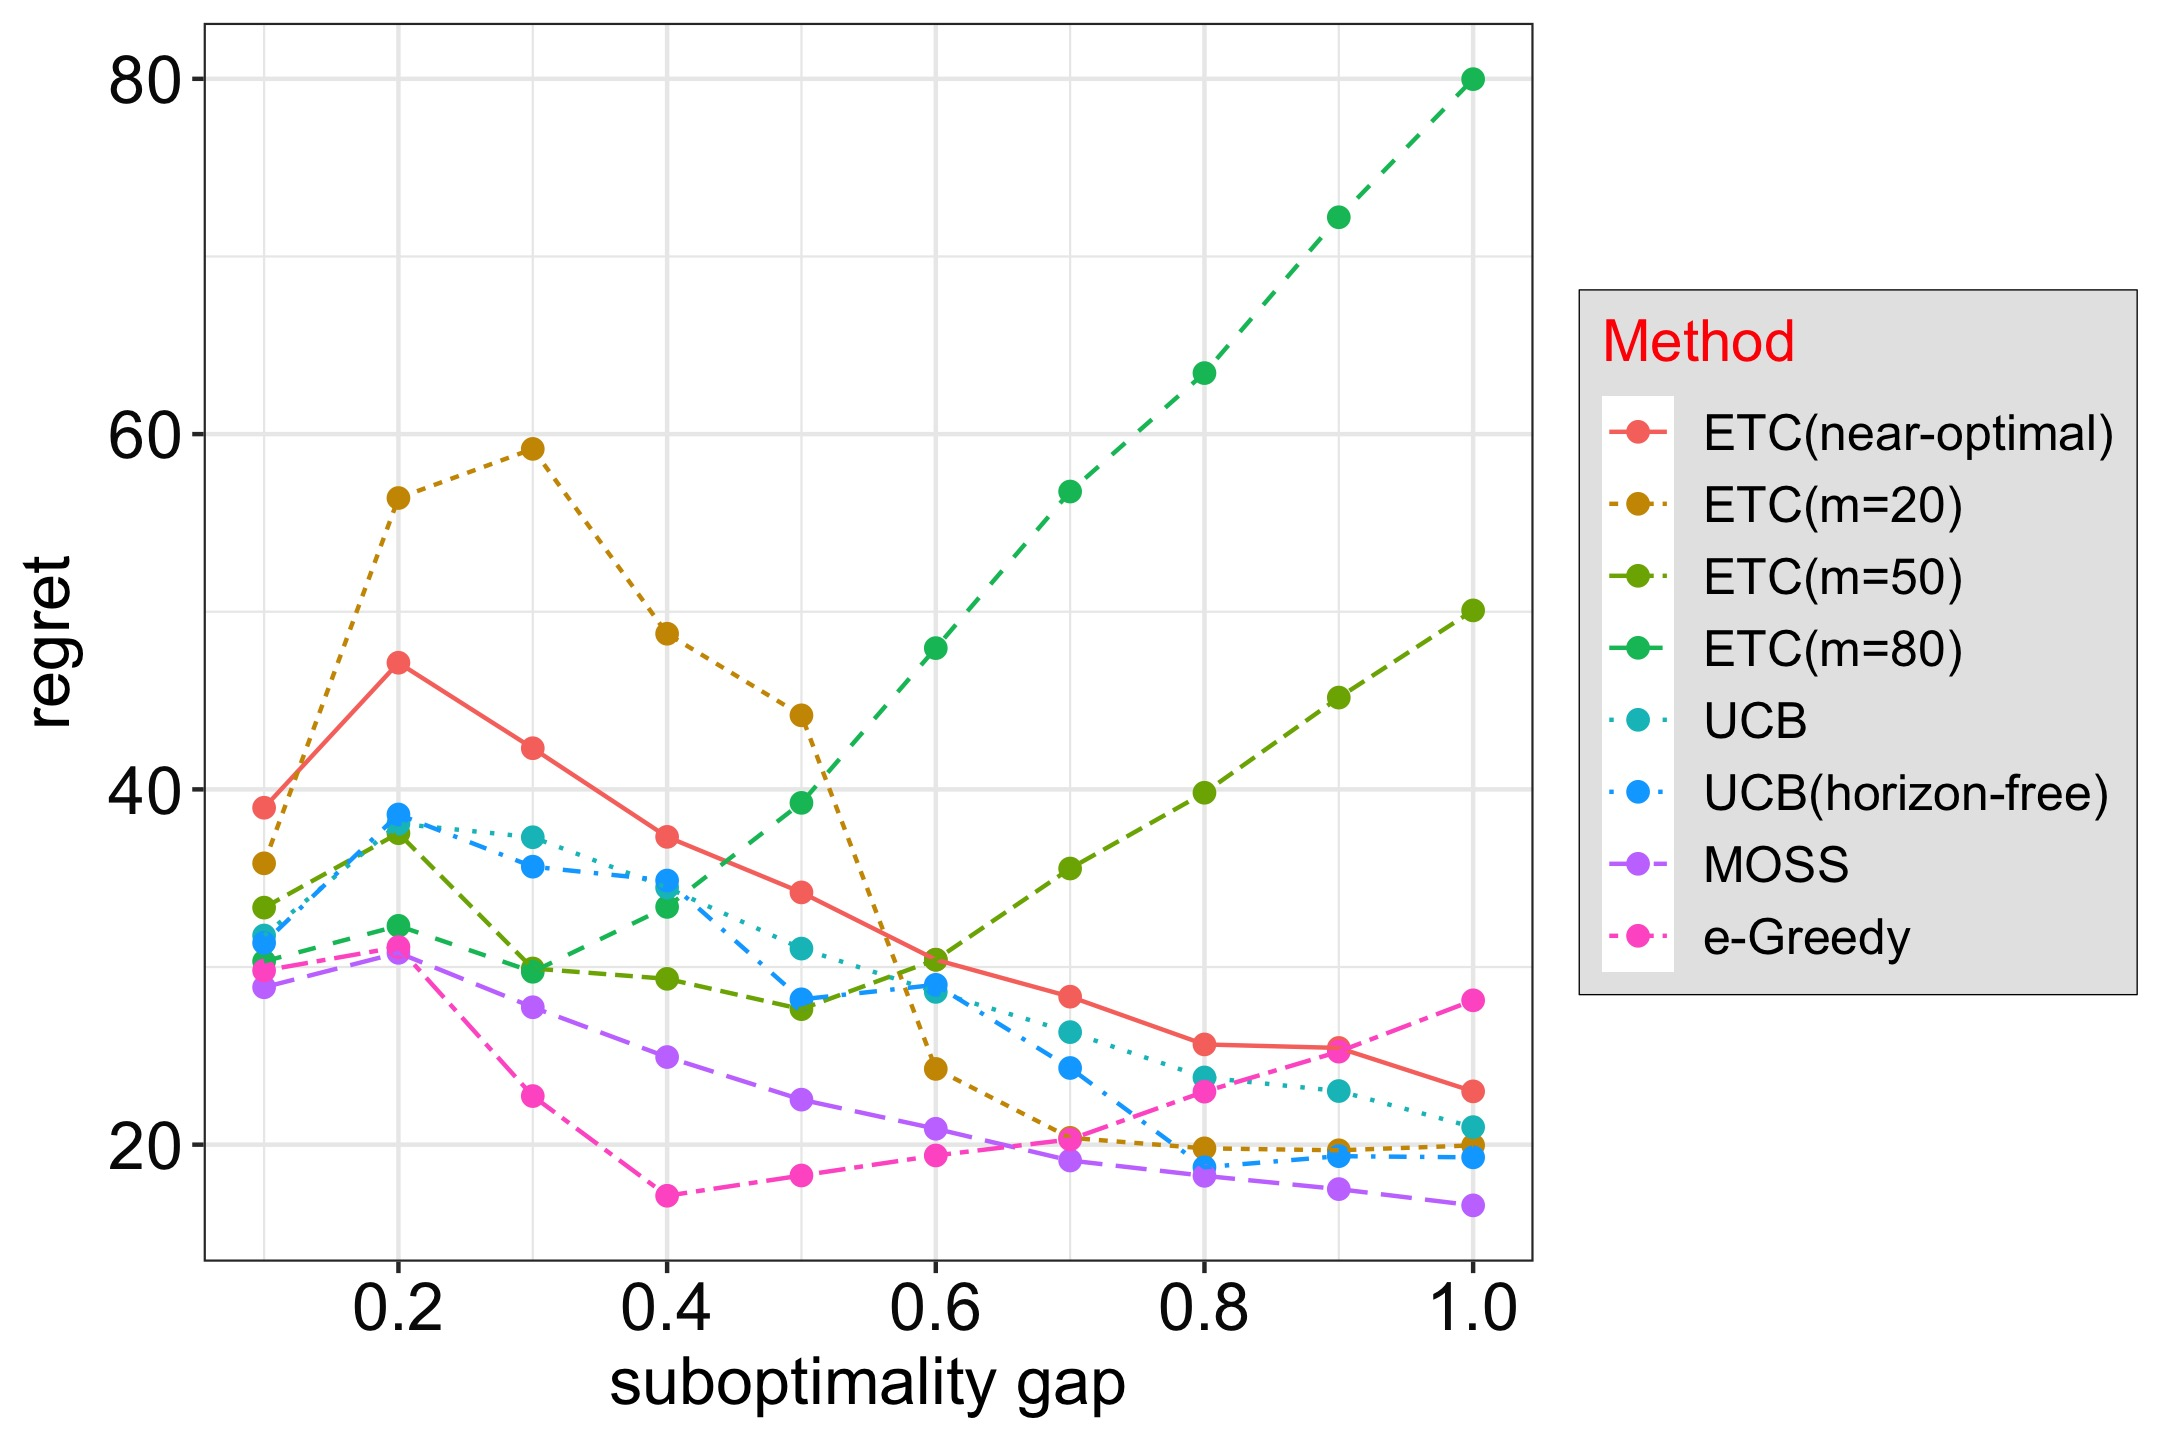
\includegraphics[width = 0.55\textwidth,clip,trim = 1cm 0cm 0cm 0cm]{sb}
\caption{Numerical simulations of several stochastic learning policies for two-armed Gaussian bandits with varying suboptimality gap.}
  \label{fig:1}
\end{figure}



\subsection{Lower bounds on regret}

To see how good the regret bounds derived in Algorithm \ref{alg:ETC} and \ref{alg:UCB}, we introduce the \emph{minimax} lower bound to quantify the comparison. Let $\V$ be the environment class, or equivalently, the set of admissible distributions on rewards: $\otimes_{i\in [k]}\nu_i$. The worst-case regret for a policy $\pi$ is defined as 
\begin{align*}
R_n(\pi, \V):=\sup_{\otimes_{i\in [k]}\nu_i\in\V}R_n(\pi).
\end{align*}
The minimax regret $R_n^*$ is the best worst-case regret among all possible policies $\Pi$: 
\begin{align}
R_n^*:=\inf_{\pi\in\Pi}R_n(\pi, \V).\label{s:mm}
\end{align}
Obtaining lower bounds on \eqref{s:mm} helps us understand the limit in stochastic bandits learning. We introduce a natural way to approach this problem.  The general idea is to show that for any $\pi\in\Pi$, there exist two environments $\nu, \nu'\in\V$ such that $R_{n,\nu}(\pi)$ and $R_{n,\nu'}(\pi)$ cannot be both small at the same time. Intuitively, a good instance for $\nu$ is bad for $\nu'$, and vice versa. If $\V$ is a parametric family, this implies that the parameter of $\nu$ is distant from the parameter of $\nu'$. On the other hand, $\pi$ should not distinguish $\nu$ from $\nu'$ so that $\E_\nu\approx\E_{\nu'}$, which requires $\nu$ to be close to $\nu'$. The right construction of $\nu$ and $\nu'$ is therefore relying on finding a trade-off point.  
\begin{Th}\label{s:minimax}
Let $\V$ be the class of normalized Gaussian bandits with mean $\mu=(\mu_i)_{i\in [k]}\in [0,1]^k$. Suppose that $n\geq k-1$. Then for any policy $\pi$ there exists some $\nu\in\V$ such that
\begin{align}
R_{n,\nu}(\pi)\geq\frac{1}{27}\sqrt{(k-1)n}. \label{s:6}
\end{align}  
\end{Th}
\begin{proof}
Fix a policy $\pi$. Let $\Delta\in [0, 1/2]$ be some parameter to be tuned later. Consider two bandits defined as
\begin{align*}
\nu &= (\Delta, 0, \cdots, 0)\\
\nu' &= (\Delta, 0, \cdots, \underbrace{2\Delta}_{\text{$i$-th component}}, 0, \cdots, 0),
\end{align*}
where $i$ is the least-played arm by $\nu$ on average: $i=\arg\min_{j>1}\E_\nu[T_j(n)]$. It is clear that spending too much time on arm $1$ is good for $\nu$ but bad for $\nu'$. Precisely, using the Chebyshev's inequality,
\begin{align}
R_{n, \nu}(\pi)+R_{n, \nu'}(\pi)\geq \frac{n\Delta}{2}\left(\P_\nu\left(T_1(n)\leq \frac{n}{2}\right)+\P_{\nu'}\left(T_1(n)> \frac{n}{2}\right)\right).\label{s:3}
\end{align}
The right-hand side of \eqref{s:3} can be bounded via Le Cam's method in statistics. A convenient form is to use the Bretagnolle-Huber inequality, which states that for probability measure $\P$ and $\Q$ on the same probability space $(\Omega, \mathcal{F})$, and $A\in\mathcal{F}$, 
\begin{align}
\P(A)+\Q(A^c)\geq\frac{1}{2}\max\left\{e^{-\textsf D_{KL}(\P||\Q)}, e^{-\textsf D_{KL}(\Q|| \P)}\right\},\label{s:4}
\end{align}
where $\textsf D_{KL}(\cdot || \cdot)$ is the KL-divergence. Let $A = \{T_1(n)\leq n/2\}$, and $\P, \Q$ be the $\pi$-induced measure on $([k]\oplus\R)^n$ under $\nu$ and $\nu'$, respectively. It can be checked by definition that 
\begin{align}
\textsf D_{KL}(\P, \Q)& = \sum_{j\in [k]}\E_\nu[T_j(n)]\textsf D_{KL}(\mu_j, \mu'_j)\label{s:5}\\
& = \E_\nu[T_i(n)]\textsf D_{KL}(\mu_i, \mu'_i)\nonumber\\
& \leq\frac{2n}{k-1}\Delta^2\nonumber,
\end{align}
where the last inequality follows from the fact that $\sum_{j\in [k]}\E_\nu[T_j(n)]=n$. Plugging \eqref{s:4} and \eqref{s:5} into \eqref{s:3} yields
\begin{align*}
R_{n, \nu}(\pi)+R_{n, \nu'}(\pi)\geq\frac{n\Delta}{4}e^{-\frac{2n\Delta^2}{k-1}}. 
\end{align*}
Taking $\Delta = \sqrt{\frac{k-1}{4n}}$ gives the desired result. 
\end{proof}
The constant $1/27$ in the bound \eqref{s:6} can be improved to $1/8$ via a different approach, which considers a sequence of environment instead of two, that are mutually inconsistent. The rest of the proof goes similarly by using the Pinsker's inequality.   

Theorem \ref{s:minimax} may be conservative if one is only interested in lower bounds on a set of `good' policies. In this case, one may derive a stronger result on the asymptotic behaviour of the regret appealing to \emph{instance-dependent} analysis, which is presented as follows.  

First of all, let us clarify what the good policies are. A policy $\pi$ is \emph{consistent} over $\V$ if for all $\nu\in\V$ and $p>0$, 
\begin{align*}
\lim_{n\rightarrow\infty}\frac{R_{n, \nu}(\pi)}{n^p} = 0. 
\end{align*}
Roughly speaking, the regret of a consistent policy is of logarithmic order asymptotically. Denote by $\Pi_{c}(\V)$ the set of consistent policies over $\V$. The following theorem implies that such intuition is accurate in a strong sense. 

\begin{Th}\label{s:ins}
Let $\nu\in\V = \otimes_{i\in [k]} \V_i$ and $1$ be the optimal arm. For any $\pi\in\Pi_c(\V)$,
\begin{align}
\liminf_{n\rightarrow\infty}\frac{R_{n,\nu}(\pi)}{\log n}\geq \sum_{i: \Delta_i>0}\frac{\Delta_i}{\mathsf d_{\inf} (\mu_i, \mu_1, \V_i)}, 
\end{align}
where $\mathsf d_{\inf} (\mu_i, \mu_1, \V_i) = \inf_{\nu_i'\in\V_i, \mu_i'>\mu_1}\textsf D_{KL}(\nu_i, \nu_i')$. 
\end{Th}
\begin{proof}
The idea of the proof is similar to Theorem \ref{s:minimax}. Thanks to \eqref{s:2} it suffices to prove that for $i\in [k]$ with nonzero suboptimality gap, 
\begin{align*}
\E_\nu[T_i(n)]\geq \mathsf d^{-1}_{\inf} (\mu_i, \mu_1, \V_i).
\end{align*}
To show this, consider a modified bandit $\nu'$ that agrees with $\nu$ except at the $i$-th arm, which equals $\nu_i'\in\V_i$ such that $\textsf D_{KL}(\nu_i, \nu_i') < \mathsf d_{\inf} (\mu_i, \mu_1, \V_i)+\e$ for some $\e>0$. Applying the Bretagnolle-Huber inequality with $A = \{T_i(n)\leq n/2\}$ and $\P, \Q$ the $\pi$-induced measure on $([k]\oplus\R)^n$ under $\nu$ and $\nu'$, respectively, 
\begin{align}
R_{n, \nu}(\pi)+R_{n, \nu'}(\pi)\geq\frac{n}{2}\min\{\Delta_i, \mu_i'-\mu_1\}e^{-(\mathsf d_{\inf} (\mu_i, \mu_1, \V_i)+\e)\E_\nu[T_i(n)]}.\label{s:7}
\end{align}
The left-hand side of \eqref{s:7} can be further bounded from above since $\pi$ is consistent. Indeed, for any $p>0$, there exists an absolute constant $c_p$ such that $R_{n, \nu}(\pi)+R_{n, \nu'}(\pi)<c_pn^p$. Plugging this in \eqref{s:7} and taking $n$, $\e$ and $p$ to $\infty$, $0$ and $0$ sequentially produces the desired result. 
\end{proof}
Theorem \ref{s:ins} is more of theoretical interest, as the asymptotic result often hides the worrying constants that matter in practice. However, from this point of view, it can be checked that MOSS is asymptotically optimal in the $1$-subgaussian environment.   


\section{Stochastic linear bandits}

\subsection{Stochastic contextual bandits and stochastic linear bandits}

Contextual structures can be made of good use in bandit learning. To incorporate such side-information, we further assume that players have access to the present context before selecting an arm in each round. Precisely, let $\mathcal C$ be the set of contexts and $\pi=(\pi_t)_{t\in [n]}\in [k]^n$ be a policy. $\pi_t$ is measurable with respect to the past decisions/rewards as well as the contexts revealed up to time $t$. The rewards collected by the player are 
\begin{align}
x_{t} = r(c_t, \pi_t)+\eta_{t}\ \ \ \ \ \ t\in [n],\label{sl:1}
\end{align}
where $c_t\in\mathcal C$ (deterministic or random) is the context in round $t$, $r(\cdot, \cdot):\mathcal C\times [k]\to\R$ is the reward function, and $\eta_{t}$ is the noise satisfying 
\begin{align}
\E[e^{\lambda\eta_{t}}|c_{1}, \pi_{1}, x_{1}, \cdots, c_{t}, \pi_{t}]\leq e^{\lambda^2/2}. \label{sl:2}
\end{align}
It is easy to check from \eqref{sl:2} that $\eta_t$ is subgaussian conditional on the history. \eqref{sl:1} and \eqref{sl:2} together lead to the so-called \emph{stochastic contextual bandits}. Due to the lack of knowledge of $r$, the regret is characterized by 
\begin{align}
R_n = \underbrace{\E\left[\sum_{c\in\mathcal C}\sum_{t: \pi_t = c}\max_{i\in [k]}r(c, i)\right]}_{(*)} - \E\left[\sum_{t\in [n]}x_{t}\right]. \label{sl:reg}
\end{align}
$(*)$ implicitly agrees that the best policy in each round is to play the arm with the largest expected reward in the present context, which is most meaningful if the dependence between contexts and actions is mild. A counterexample is when an optimal action at the beginning leads to unfavorable contexts in the subsequent rounds. The ideal $c_t$ under our consideration is either deterministic or independent of the past actions.  Conditional on $(c_t)_{t\in [n]}$, $R_n$ becomes a sum of regrets of $|\mathcal C|$ stochastic bandits. Heuristically, the best strategy is to treat the contexts separately and apply the optimal policy for each individual,  
\begin{align}
R_n=\E\left[\sum_{c\in\mathcal C}\E\left[R_{n,c}|c_1, \cdots, c_n\right]\right]\stackrel{\text{Thm.}\ \ref{s:ins}}{\lesssim}\E\left[\sum_{c\in\mathcal C}\sqrt{k\sum_{t\in [n]}\mathbb I_{c_t = c}}\right]\leq\sqrt{nk|\mathcal C|}.\label{sl:3}
\end{align} 
This immediately generalizes the results in Section \ref{sec1} to the stochastic contextual bandits, assuming nothing on the reward function $r$. However, in some practical situations, $|\mathcal C|$ can be astronomical (i.e., $|\mathcal C|>>\sqrt{n}$), making \eqref{sl:3} a vacuous bound.  The problem here is that our strategy only uses the combinatorial nature of $\mathcal C$. For example, supposing that $\mathcal C$ is a subset of a normed space and $r$ is continuous, one would expect $r(c, \cdot)$ and $r(c', \cdot)$ to be close if $||c-c'||$ is small. Yet this is not utilized in the above algorithm design which deals with elements in $\mathcal C$ in parallel. To utilize other information of $\mathcal C$, we could further hypothesize on the structures of $r$ (i.e., $r$ is in some parametric family). A simple choice gives rise to a class of interesting models which we will study next. 

Suppose that $r(c,i)$ is a linear function of a high-dimensional feature determined by $(c, i)$ via a kernel map $\phi(c,i): \mathcal C\times [k]\to\R^d$. That is, $r(c, i) = \langle\t, \phi(c,i) \rangle$ for some $\t\in\R^d$. In this case \eqref{sl:reg} can be rewritten as 
\begin{align}
R_n = \E\left[\sum_{t\in [n]}\max_{a\in\mathcal A_t}\langle\theta, a\rangle-x_{t}\right],\label{sl:4}
\end{align}  
where $\mathcal A_t = \{\phi(c_t, i)\}_{i\in [k]}$ is the set of features available at time $t$. Here $\theta$ is unknown, and $\mathcal A_t$ is a finite set which can be either deterministic or random. This particular parametrization of $r$ is called \emph{stochastic linear bandits}. 

We next discuss a few policies in stochastic linear bandits, depending on different assumptions on $\mathcal A_t$. Note that $\mathcal A_t$ is finite from the perspective of stochastic contextual bandits and the kernel map. However, in the general set-up of stochastic linear bandits, $\mathcal A_t$ is allowed to be infinite. Regardless of varying assumptions on $\mathcal A_t$, the regret defined in \eqref{sl:4} is based on the lack of information of $r$ so that one always needs to efficiently estimate for $\theta$ in the exploration process. Nevertheless, the efficiency here can have different meanings for different types of $\mathcal A_t$, which needs to be discussed in a case-dependent manner. 

\subsection{Stochastic linear bandits: fixed and finite action sets}

We begin our analysis for stochastic linear bandits whose action set $\mathcal A_t = \mathcal A$ does not change with time. We also assume that $|\mathcal A|=k$. Let $a_t\in\mathcal A$ be the feature vector associated with the action under some policy $\pi$ at time $t$. The exploration process suffices to estimate $\t$, and a natural estimator is the least-squares estimator. One may use the Ridge estimator if having invertibility issues. Precisely, in round $t$, $\t$ is estimated by $\hat{\t}_t$, where $\hat{\t}_t $ solves the normal equations: 
\begin{align*}
\underbrace{\begin{pmatrix}
a_1, \cdots, a_{t-1}
\end{pmatrix}}_{A^T_{t-1}}\underbrace{\begin{pmatrix}
a_1^T \\
\vdots \\
a_{t-1}^T
\end{pmatrix}}_{A_{t-1}}\t = \underbrace{\begin{pmatrix}
a_1, \cdots, a_{t-1}
\end{pmatrix}}_{A^T_{t-1}}\begin{pmatrix}
x_1 \\
\vdots \\
x_{t-1}
\end{pmatrix}.
\end{align*}
Note that the design matrix $A_{t-1}$ depends on the past actions. Since $\mathcal A$ is fixed, a good policy in the exploration stage should efficiently estimate the marginals of $\t$ along the directions in $\mathcal A$. In other words, for any $\e, \delta>0$, we wish to find a $\pi$ such that 
\begin{align}
T_{\pi}(\e, \delta):=\inf\left\{t: \max_{a\in\mathcal A}\underbrace{\P\left(|\langle\hat{\t}_t-\t, a\rangle|>\e\right)\leq\delta}_{\textcolor{blue}{\text{used to build c.i. for}\ \langle\t, a\rangle}}\right\}\label{sl:5}
\end{align}
is as small as possible. This is equivalent to the optimal experimental design problem in statistics. 
To see this, note that for fixed $a\in\mathcal A$, 
\begin{align*}
\P\left(|\langle\hat{\t}_t-\t, a\rangle|>\sqrt{2||a||^2_{V_{t-1}^{-1}}\log\left(\frac{2}{\delta}\right)}\right)\leq\delta,
\end{align*}
where $V_{t-1} = A^T_{t-1}A_{t-1}$. Setting 
\begin{align*}
\sqrt{2||a||^2_{V_{t-1}^{-1}}\log\left(\frac{2}{\delta}\right)}\leq\e
\end{align*}
and solving for $t$ yields
\begin{align*}
||a||_{V_{t-1}^{-1}}\leq\sqrt{\frac{\e^2}{2}\log^{-1}\left(\frac{2}{\delta}\right)}.
\end{align*}
Since $V_t^{-1}\preceq V^{-1}_{t-1}$, an upper bound for \eqref{sl:5}, which we denote by the same notation, is
\begin{align}
T_{\pi}(\e, \delta) = \inf\left\{t: \max_{a\in\mathcal A}||a||_{V_{t-1}^{-1}}\leq \sqrt{\frac{\e^2}{2}\log^{-1}\left(\frac{2}{\delta}\right)}\right\}.\label{sl:6}
\end{align}
Let $\mathcal P(\mathcal A)$ be set of probability measures on $\mathcal A$. There is a one-to-one correspondence between policies and $\mathcal P(\mathcal A)$ asymptotically (The frequency of choosing an action $a$ in $t$ rounds under $\pi$ can be roughly viewed as the probability $p(a)$). Denote by $p$ the probability measure associated with $\pi$. It is easy to verify that 
\begin{align*}
T_{\pi}(\e, \delta) = \frac{\max_{a\in\mathcal A}||a||^2_{A^{-1}(p)}}{\frac{\e^2}{2}\log^{-1}\left(\frac{2}{\delta}\right)}+1\ \ \ \ \ A(p):=\E_p[aa^T]
\end{align*}
Hence, as $t\to\infty$, minimizing \eqref{sl:6} over the possible policies is equivalent to the following optimization problem:
\begin{align}
\min_{p\in\mathcal P(\mathcal A)}\max_{a\in\mathcal A}||a||^2_{A^{-1}(p)}.\label{sl:7}
\end{align}
The term $\max_{a\in\mathcal A}||a||^2_{A^{-1}(p)}$ is often denoted by $g(p)$, and \eqref{sl:7} is referred to as the \emph{G-optimal design problem}. Solving \eqref{sl:7} relies on the following theorem due to Kiefer and Wolfowitz:
\begin{Th}[Kiefer-Wolfowitz, 1960]\label{KW}
Let $\mathcal A\subset\R^d$ be a compact set and $\text{span}(\mathcal A)=\R^d$. Then
\begin{align*}
p^*\text{solves \eqref{sl:7}}\Longleftrightarrow p^*\in\argmax_{p\in\mathcal P(\mathcal A)}\log\det A(p)\Longleftrightarrow g(p^*) = d. 
\end{align*}
Moreover, there exists a $p^*$ such that $\text{supp}(p^*)\leq d(d+1)/2$. 
\end{Th}
\begin{Rem}
The geometric interpretation of the set $\left\{||x||_{A^{-1}(p^*)}\leq d\right\}$ based on duality is the minimum volume enclosing ellipsoid for the set $\mathcal A$. When $\mathcal A$ is convex, this is known as \emph{John's ellipsoid}.  
\end{Rem}
\begin{Rem}
According to Theorem \ref{KW}, solving the $G$-optimal design problem is the same as finding the maximizer for $\log\det A(p)$, which is a convex optimization problem and can be approximately solved via Frank-Wolfe algorithm: For $a\in\mathcal A$ and $a_k = \argmax_{a\in\mathcal A}||a||_{A^{-1}(p_k)}^2$, 
\begin{align*}
p_{k+1}(a) = \left(1-\frac{\frac{1}{d}||a_k||_{A^{-1}(p_k)}-1}{||a_k||_{A^{-1}(p_k)}-1}\right)p_k(a) + \frac{\frac{1}{d}||a_k||_{A^{-1}(p_k)}-1}{||a_k||_{A^{-1}(p_k)}-1}\mathbb I_{a=a_k}.
\end{align*}
If $p_0$ is a uniform distribution on $\mathcal A$, then $g(p_k)\leq (1+\e)d$ for $k=\mathcal O(d\log\log |\mathcal A|+d/\e)$.
\end{Rem}

Once \eqref{sl:7} is (approximately) solved, one can use the solution to construct a near-optimal policy for exploration. Algorithms in Section \ref{sec1} like ETC naturally extend to this case. However, similar problems still exist as the best trade-off point usually depends on the suboptimality gaps. An alternative approach is to take the exploration adaptively together with a phase-elimination process, which is given below:

\begin{algorithm}
\DontPrintSemicolon
 \KwIn{Action set $\mathcal A$ and $\delta$.}
 \KwOut{ $\{a_t\}_{t\in [n]}.$}
 \textbf{Initialization}: $\ell = 0$, $\mathcal A_1 = \mathcal A$, $T_0 = 0$, $d_0=d$ and $N_0 = 0$.\\
 \While{$N_\ell\leq n$}{
 \begin{itemize}
 \item $\ell = \ell + 1$;
 \item $\e_\ell = 2^{-\ell}$;
 \item $p_\ell \in\argmax_{p\in\mathcal P(\mathcal A_\ell)}\log\det \mathcal A_\ell(p)$ and $\text{supp}(p_\ell)\leq d_{\ell-1}(d_{\ell-1}+1)/2$;
 \item $d_\ell = \min\{|\mathcal A_\ell|, d\}$.
 \end{itemize}
 \For{$a\in\mathcal A_\ell$}{
 $T_\ell(a)=\displaystyle\left\lceil 2\e_\ell^{-2}d_\ell p_\ell(a)\log\left(\frac{2k^2\ell(\ell+1)}{\delta}\right)\right\rceil$.}
\begin{itemize}
\item $T_\ell = \sum_{a\in\mathcal A}T_\ell(a)$;
\item For $t\in [T_{\ell-1}+1,T_\ell]$ choose action $a\in\mathcal A_\ell$ $T_\ell(a)$ times. Denote the  design matrix by $A_\ell$. 
\item $\hat{\t}_\ell = (A^T_\ell A_\ell)^{-1}A_\ell^T(x_{T_{\ell-1}+1}\cdots, x_{T_\ell})^T$;
\item $\mathcal A_{\ell+1} = \{a\in\mathcal A_\ell, \max_{b\in\mathcal A_\ell}\langle\hat{\t}_\ell, b-a\rangle\leq 2\e_\ell\}$; 
\item $N_\ell = N_{\ell-1} + T_\ell$. 
\end{itemize}
}
\caption{Phase-elimination with $G$-optimal exploration algorithm. } 
\label{alg:sl-finite}
\end{algorithm}

Assume additionally that the largest suboptimality gap is bounded by $1$. Then the regret analysis of Algorithm \ref{alg:sl-finite} can be summarized in the following theorem:

\begin{Th}\label{sl:finite}
The psudo-regret $\bar{R}_n=n\max_{a\in\mathcal A}\langle\t, a\rangle-\sum_{t\in [n]}\langle\t, a_t\rangle$ in Algorithm \ref{alg:sl-finite} satisfies
\begin{align*}
\P\left(\bar{R}_n> 32\left(\sqrt{nd\log\left(\frac{k\log n}{\delta}\right)}+d^2\right)\right)\leq \delta, 
\end{align*}
\end{Th}
Moreover, integrating the tail probability,
\begin{align*}
R_n\leq 64(\sqrt{nd\log (k\log n)}+d^2). 
\end{align*}
\begin{proof}
Algorithm \ref{alg:sl-finite} guarantees a high probability that (i). an optimal action $a^*$ is always in $\mathcal A_\ell$ , and (ii). suboptimal arms can only survive finitely many times. In fact, 
\begin{align*}
&\P\left(a^*\in\mathcal A_\ell\  \text{for only finitely many}\ \ell \right)\\
\leq&\ \  \sum_{\ell\in\N}\P\left(a^*\notin\mathcal A_{\ell+1}|a^*\in\mathcal A_{\ell}\right)\\
\leq&\ \ \sum_{\ell\in\N}\sum_{\substack{a\in\mathcal A_\ell\\ a\neq a^*}}\left(\P\left(|\langle\hat{\t}_{\ell+1}-\t, a^*\rangle|>\e_{\ell+1}\right)+\P\left(|\langle\hat{\t}_{\ell+1}-\t, a\rangle|>\e_{\ell+1}\right)\right)\leq\frac{\delta}{k}.
\end{align*}
On the other hand, let $\Delta_a = \langle\t, a^*-a\rangle$ be the suboptimality gap between $a$ and $a^*$ and define $\ell_a = 2+\lceil\log\Delta_\ell^{-1}\rceil$ (base 2). Then, 
\begin{align*}
\P\left(a\in\mathcal A_{\ell_a}\right)&\leq \P\left(|\langle\hat{\t}_{\ell_a}-\t, a^*\rangle|>\e_{\ell_a}\right)+\P\left(|\langle\hat{\t}_{\ell_a}-\t, a\rangle|>\e_{\ell_a}\right)\leq \frac{\delta}{k}. 
\end{align*}
Taking a union bound gives
\begin{align}
\P\left(a^*\in\bigcap_{\ell\in\N}\mathcal A_\ell\ \&\ a\notin \mathcal A_{\ell_a}\ \text{for all $a\in\mathcal A$ with $\Delta_a>0$} \right)\geq 1-\delta. \label{sl:8}
\end{align}
We now estimate $\bar{R}_n$ conditional on the event defined in \eqref{sl:8}. Let $\Delta>0$ be some parameter to be tuned later. We first consider the actions played in the first $n$ rounds with suboptimality gap less than $\Delta$. It is clear that the cumulative loss incurred by these actions is bounded by $n\Delta$. On the other hand, the actions with suboptimality gap greater than $\Delta$ can be played only in the first $\ell_\Delta$ rounds, where $\ell_\Delta = 1+\lceil\log\Delta^{-1}\rceil\leq 2+\log\Delta^{-1}$. The regret of these actions is bounded by the total loss incurred in first $\ell_\Delta$ rounds of exploration, which is further bounded by  
\begin{align*}
\sum_{\ell = 1}^{\log n\wedge \ell_\Delta}4\e_\ell T_\ell &\leq \frac{64}{\Delta}d\log\left(\frac{4k^2\log^2 n}{\delta}\right) + 4d^2,
\end{align*} 
where for $\ell=1$ we used that the maximum of suboptimality gaps is less than $1\leq 4\e_1$. Therefore, 
\begin{align*}
\bar{R}_n&\leq\inf_{0<\Delta<1}\left\{n\Delta+\frac{64}{\Delta}d\log\left(\frac{4k^2\log^2 n}{\delta}\right)+4d^2\right\}\\
&\leq 16\sqrt{nd\log\left(\frac{4k^2\log^2 n}{\delta}\right)}+4d^2\\
&\leq 32\left(\sqrt{nd\log\left(\frac{k\log n}{\delta}\right)}+d^2\right). 
\end{align*}
The proof is thus complete. 
\end{proof}
\begin{Rem}
One advantage of Algorithm \ref{alg:sl-finite} is that it behaves well even when the model is misspecified. Particularly, if the observation $x_t$ is contaminated by some noise of magnitude less than $\e$, then it can be proved that 
\begin{align*}
R_n=\mathcal O\left(\sqrt{nd\log (kn)}+\e n\sqrt{d}\log n\right). 
\end{align*}
\end{Rem}

\begin{Rem}
Taking $\mathcal A$ as canonical bases in $\R^d$ and $d=k$,  Algorithm \ref{alg:sl-finite} reduces to an elimination algorithm for stochastic bandits. Theorem \ref{sl:finite} tells us that the asymptotic regret is $\mathcal O(\sqrt{nk\log\log n})$.   
\end{Rem}

\subsection{Stochastic linear bandits: general action sets}











 
\printbibliography
 
 
\end{document}